\section{Introducing differentiable binary arithmetic operations}
\label{sec:Nalu}
Our goal is to achieve arithmetic operations between the elements of a vector. Such that the output is an addition, subtraction, multiplication, or division of arbitrary elements of a vector $\mathbf{x}$ (e.g. ${x_5 + x_1 \cdot x_7}$). Formally defined as
\begin{equation}
x_1\circ_1 x_2 \circ_2 \cdots x_{k-1} \circ_{k-1} x_{k}\ |\ (x_1, \dots, x_k) \in \mathbf{x}, \mathbf{x} \in \mathbb{R}^n, \circ_i \in \{+, -, \times, \div \}
\label{eq:goal}
\end{equation}

The Neural Arithmetic Logic Unit (NALU) \cite{trask-nalu} attempts to solve equation \ref{eq:goal} by presenting two sub-units; the $\text{NAC}_{+}$ and $\text{NAC}_{\bullet}$ to exclusively represent either the $\{+, -\}$ or the $\{\times, \div \}$ operations.
The NALU attempts to have either $\text{NAC}_{+}$ or $\text{NAC}_{\bullet}$ selected exclusively, which could require the NALU to be applied multiple times (alternating between $\text{NAC}_{+}$ and $\text{NAC}_{\bullet}$) in order to represent the entire space of solutions for equation \ref{eq:goal}.

The $\text{NAC}_{+}$ and $\text{NAC}_{\bullet}$ are defined accordingly,

\begin{align}
W_{h_\ell, h_{\ell-1}} &= \tanh(\hat{W}_{h_\ell, h_{\ell-1}}) \sigma(\hat{M}_{h_\ell, h_{\ell-1}}) \label{eq:weight}\\
\textrm{NAC}_+:\ z_{h_\ell} &= \sum_{h_{\ell-1}=1}^{H_{\ell-1}} W_{h_{\ell}, h_{\ell-1}} z_{h_{\ell-1}} \label{eq:naca}\\
\textrm{NAC}_\bullet:\ z_{h_\ell} &= \exp\left(\sum_{h_{\ell-1}=1}^{H_{\ell-1}} W_{h_{\ell}, h_{\ell-1}} \label{eq:nacm}\log(|z_{h_{\ell-1}}| + \epsilon) \right)
\end{align}
where $\hat{\mathbf{W}}, \hat{\mathbf{M}} \in \mathbb{R}^{H_{\ell} \times H_{\ell-1}}$ are trainable weight matrices. The matrices are combined using tanh and sigmoid transformation to bias the parameters towards a $\{-1,0,1\}$ solution. Having $\{-1,0,1\}$ allows a linear layer to exactly emulate the binary $\{+, -\}$ operation between elements of a vector as used when computing the $\text{NAC}_{+}$.
The $\text{NAC}_{\bullet}$ extends the $\text{NAC}_{+}$ by using an exponential log transformation, which, with $\{-1,0,1\}$ weight values, becomes the $\{\times, \div \}$ operations (within $\epsilon$ precision).

The NALU combines these units with a gating mechanism $\mathbf{z} = \mathbf{g} \odot \text{NAC}_{+} + (1 - \mathbf{g}) \odot \text{NAC}_{\bullet}$ given $\mathbf{g} = \sigma(\mathbf{G} \mathbf{x})$. The idea is that the NALU should be a plug-and-play component in a neural network and has the ability to, with stochastic gradient descent and backpropagation, to learn the functionality in equation \ref{eq:goal}.

\subsection{Challenges of the NALU, $\text{NAC}_{+}$ and $\text{NAC}_{\bullet}$}
To simplify the problem we have chosen to leave out the gating mechanism and focus on the sub-units, assuming "oracle gating". We have not had any consistent success of convergence using the gating mechanism using the NALU or by combining our own proposed sub-units (NAU, NMU), as shown in table \ref{tab:function-task-static-defaults}. We find that gating between $\text{NAC}_{+}$ and $\text{NAC}_{\bullet}$ is challenging. This is likely due to the vastly different gradients, causing addition to be learned much faster than multiplication.

%In section \ref{sssec:weight} we analyse the gradients of equation \ref{eq:weight} and propose a cliped linear alternative, with a regularizer that biases towards $\{-1, 0, 1\}$. This results in an alternative addition unit called NAU.

%In section \ref{sssec:nac-mul} we analyse the gradient of $\text{NAC}_{\bullet}$, and propose an alternative construction called NMU, that has a more well-behaved loss space.

%In section \ref{sssec:nac-add-moments} we analyse the moments of $\text{NAC}_{+}$ and NAU, and derive the optimal weight initializations.

%In section \ref{sssec:nac-mul-moments} we analyse the moments of $\text{NAC}_{\bullet}$ and NMU, and show that the NMU have a more well-behaved expectation and variance. \todo{Maybe remove this overview?}

\subsubsection{Weight matrix construction}\label{sssec:weight}

The weight matrix construction $\mathrm{tahn}(\hat{W}_{h_{\ell-1},h_\ell}) \sigma(\hat{M}_{h_{\ell-1},h_\ell})$ has the following properties that could make convergence challenging using gradient decent.

The loss gradient with respect to the weight matrices can be derived from equation \ref{eq:weight}.
\begin{equation}
\begin{aligned}
\frac{\partial \mathcal{L}}{\partial \hat{W}_{h_{\ell-1},h_\ell}} &= \frac{\partial \mathcal{L}}{\partial W_{h_{\ell-1},h_\ell}} (1 - \tanh^2(\hat{W}_{h_{\ell-1},h_\ell})) \sigma(\hat{M}_{h_{\ell-1},h_\ell}) \\
\frac{\partial \mathcal{L}}{\partial \hat{M}_{h_{\ell-1},h_\ell}} &= \frac{\partial \mathcal{L}}{\partial W_{h_{\ell-1},h_\ell}} \tanh(\hat{W}_{h_{\ell-1},h_\ell}) \sigma(\hat{M}_{h_{\ell-1},h_\ell}) (1 - \sigma(\hat{M}_{h_{\ell-1},h_\ell}))
\end{aligned}
\label{eq:nac-weight-gradient}
\end{equation}

The gradient $E\left[\nicefrac{\partial \mathcal{L}}{\partial \hat{M}_{h_{\ell-1},h_\ell}}\right] = 0$ can be problematic as we prefer zero having a zero mean expectation of our output.
Something that can only be ensured with $E[\hat{W}_{h_{\ell-1},h_\ell}] = 0$ \cite{glorot-initialization}.

In our empirical analysis we find that equation \ref{eq:weight} does not create the desired bias for $\{-1, 0, 1\}$, as it doesn't converge towards those values.

To create a bias and prevent the gradient challenges of equation \ref{eq:nac-weight-gradient} we propose a simple clamped linear construction with an out-of-bound regularizer $\mathcal{R}_{\ell,\mathrm{oob}}$ to force $\hat{W}$ to be within $[-1, 1]$ and ensure that the gradient is always present.
\begin{equation}
\begin{aligned}
W_{h_{\ell-1},h_\ell} &= \min(\max(\hat{W}_{h_{\ell-1},h_\ell}, -1), 1), \\
\mathcal{R}_{\ell,\mathrm{bias}} &= \frac{1}{H_\ell + H_{\ell-1}} \sum_{h_\ell=1}^{H_\ell} \sum_{h_{\ell-1}=1}^{H_{\ell-1}} \hat{W}_{h_{\ell-1},h_\ell}^2 (1 - |\hat{W}_{h_{\ell-1},h_\ell}|)^2 \\
\mathcal{R}_{\ell,\mathrm{oob}} &= \frac{1}{H_\ell + H_{\ell-1}} \sum_{h_\ell=1}^{H_\ell} \sum_{h_{\ell-1}=1}^{H_{\ell-1}} \max(|\hat{W}_{h_{\ell-1},h_\ell}| - 1, 0)^2 \\
\textrm{NAU}:\ z_{h_\ell} &= \sum_{h_{\ell-1}=1}^{H_{\ell-1}} W_{h_{\ell}, h_{\ell-1}} z_{h_{\ell-1}} \\
\mathcal{L} &= \hat{\mathcal{L}} + \lambda_{\mathrm{bias}} \mathcal{R}_{\ell,\mathrm{bias}} + \lambda_{\mathrm{oob}} \mathcal{R}_{\ell,\mathrm{oob}}
\end{aligned}
\end{equation}

\subsubsection{Challenges of division} \label{sssec:nac-mul}

The $\text{NAC}_{\bullet}$, as formulated in equation \ref{eq:nacm}, has the ability to learn exact multiplication and division of elements from a vector if the weights of $W_{h_{\ell-1},h_\ell}$ are one of $\{-1, 0, 1\}$.

However, backpropagation through the $\text{NAC}_{\bullet}$ unit reveals that if $|z_{h_{\ell-1}}|$ is near zero, $W_{h_{\ell-1},h_\ell}$ is negative and $\epsilon$ is small, the gradient term will explode and oscillate between large positive and large negative values, which can be problematic in optimization \cite{adam-optimization}, as visualized in figure \ref{fig:nac-mul-eps-issue}.

\begin{align}
%\frac{\partial \mathcal{L}}{\partial W_{h_{\ell}, h_{\ell - 1}}} &= \frac{\partial \mathcal{L}}{\partial z_{h_\ell}} \frac{\partial z_{h_\ell}}{\partial W_{h_{\ell}, h_{\ell - 1}}} = \frac{\partial \mathcal{L}}{\partial z_{h_\ell}} z_{h_\ell} \log(|z_{h_{\ell-1}}| + \epsilon) \label{eq:dw}\\
\frac{\partial \mathcal{L}}{\partial z_{h_{\ell-1}}} &= \sum_{h_\ell = 1}^{H_\ell} \frac{\partial \mathcal{L}}{\partial z_{h_\ell}} \frac{\partial z_{h_\ell}}{\partial z_{h_{\ell-1}}} = \sum_{h_\ell = 1}^{H_\ell} \frac{\partial \mathcal{L}}{\partial z_{h_\ell}} z_{h_\ell} W_{h_\ell, h_{\ell-1}} \frac{\mathrm{sign}(z_{h_{\ell-1}})}{|z_{h_{\ell-1}}| + \epsilon}\label{eq:dz}
\end{align}
(see full derivation in Appendix \ref{sec:appendix:gradient-derivatives:gradient-nac-mul})

This is not an issue for for positive values of $W_{h_{\ell-1},h_\ell}$ (multiplication), as $z_{h_{\ell}}$ and $z_{h_{\ell-1}}$ will be correlated causing the terms $z_{h_\ell}$ and $\frac{\mathrm{sign}(z_{h_{\ell-1}})}{|z_{h_{\ell-1}}| + \epsilon}$ to partially cancel out.
\begin{figure}[h]
\centering
\begin{subfigure}{.33\textwidth}
  \centering
  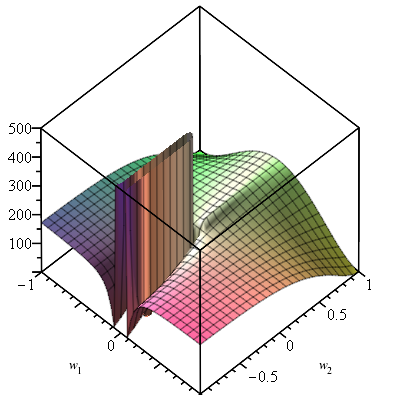
\includegraphics[width=\linewidth]{graphics/nac-mul-eps-1em7.png}
  \caption{$\mathrm{NAC}_{\bullet}$ with $\epsilon = 10^{-7}$}
\end{subfigure}%
\begin{subfigure}{.33\textwidth}
  \centering
  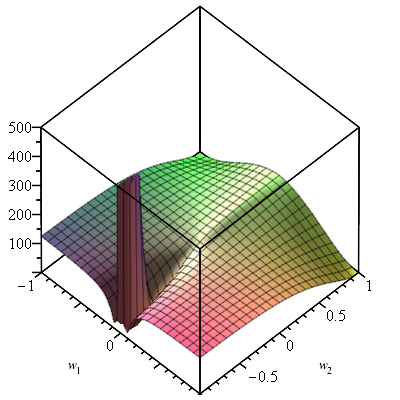
\includegraphics[width=\linewidth]{graphics/nac-mul-eps-1em1.png}
  \caption{$\mathrm{NAC}_{\bullet}$ with $\epsilon = 0.1$}
\end{subfigure}
%\begin{subfigure}{.33\textwidth}
%  \centering
%  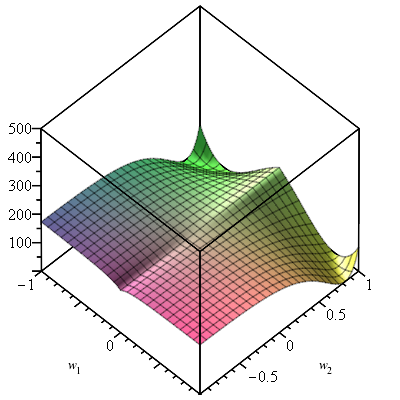
\includegraphics[width=\linewidth]{graphics/nac-mul-eps-1.png}
%  \caption{$\epsilon = 1$}
%\end{subfigure}
\begin{subfigure}{.33\textwidth}
  \centering
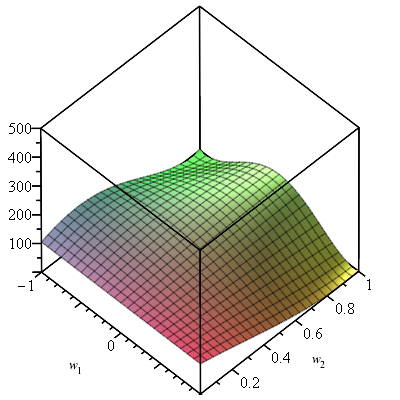
\includegraphics[width=\linewidth]{graphics/nac-mul-nmu.png}
  \caption{Our NMU solution}
\end{subfigure}

\caption{RMS loss curvature for a $\mathrm{NAC}_{+}$ layer followed by either a $\mathrm{NAC}_{\bullet}$ or NMU layer. The weight matrices constrained are to $\mathbf{W}_1 = \left[\protect\begin{smallmatrix}
w_1 & w_1 & 0 & 0 \\
w_1 & w_1 & w_1 & w_1
\protect\end{smallmatrix}\right]$, $\mathbf{W}_2 = \left[\protect\begin{smallmatrix}
w_2 & w_2
\protect\end{smallmatrix}\right]$. The problem is $x = \left(1, 1.2, 1.8, 2\right), t = 13.2$. Desired solution is $w_1 = w_2 = 1$, although this problem have additional undesired solutions.}
\label{fig:nac-mul-eps-issue}
\end{figure}

This gradient can be particular problematic when considering that $E[z_{h_{\ell-1}}] = 0$ is a desired property when initializing \cite{glorot-initialization}. An alternative multiplication operator must thus be able to not explode for $z_{h_{\ell-1}}$ near zero. To that end we propose a new neural multiplication units (NMU):

\begin{equation}
\begin{aligned}
W_{h_{\ell-1},h_\ell} &= \min(\max(\hat{W}_{h_{\ell-1},h_\ell}, 0), 1), \\
\mathcal{R}_{\ell,\mathrm{bias}} &= \frac{1}{H_\ell + H_{\ell-1}} \sum_{h_\ell=1}^{H_\ell} \sum_{h_{\ell-1}=1}^{H_{\ell-1}} \hat{W}_{h_{\ell-1},h_\ell}^2 (1 - \hat{W}_{h_{\ell-1},h_\ell})^2 \\
\mathcal{R}_{\ell,\mathrm{oob}} &= \frac{1}{H_\ell + H_{\ell-1}} \sum_{h_\ell=1}^{H_\ell} \sum_{h_{\ell-1}=1}^{H_{\ell-1}} \max\left(\left|\hat{W}_{h_{\ell-1},h_\ell} - \frac{1}{2}\right| - \frac{1}{2}, 0\right)^2 \\
\textrm{NMU}:\ z_{h_\ell} &= \prod_{h_{\ell-1}=1}^{H_{\ell-1}} \left(W_{h_{\ell-1},h_\ell} z_{h_{\ell-1}} + 1 - W_{h_{\ell-1},h_\ell} \right) \\
\mathcal{L} &= \hat{\mathcal{L}} + \lambda_{\mathrm{bias}} \mathcal{R}_{\ell,\mathrm{bias}} + \lambda_{\mathrm{oob}} \mathcal{R}_{\ell,\mathrm{oob}}
\end{aligned}
\end{equation}
Notable is the multiplicative identity for when $W_{h_{\ell-1},h_\ell}=0$.
This unit does not support division, but supporting division is likely infeasible as dividing by $z_{h_{\ell-1}}$ near zero would cause explosions.
As shown in \cite{trask-nalu}, experiments using the NALU for division does not work well hence very little is lost with this modification.
As opposed to the NALU, the NMU can represent input of both negative and positive $z_{h_{\ell-1}}$ values and is not $\epsilon$ dependent, which allows the NMU to extrapolate inputs that are negative or smaller than $\epsilon$.

The gradients with respect to the weight and input in the NMU are (see details in Appendix \ref{sec:appendix:gradient-derivatives:gradient-nmu}):
\begin{equation}
\begin{aligned}
\frac{\partial \mathcal{L}}{\partial W_{h_{\ell}, h_{\ell - 1}}} &= \frac{\partial \mathcal{L}}{\partial z_{h_\ell}} \frac{\partial z_{h_\ell}}{\partial W_{h_{\ell}, h_{\ell - 1}}} = \frac{\partial \mathcal{L}}{\partial z_{h_\ell}} \frac{z_{h_\ell}}{W_{h_{\ell-1},h_\ell} z_{h_{\ell-1}} + 1 - W_{h_{\ell-1},h_\ell}} \left(z_{h_{\ell-1}} - 1\right) \\
\frac{\partial \mathcal{L}}{\partial z_{h_{\ell-1}}} &= \sum_{h_\ell = 1}^{H_\ell} \frac{\partial \mathcal{L}}{\partial z_{h_\ell}} \frac{\partial z_{h_\ell}}{\partial z_{h_{\ell-1}}} = \sum_{h_\ell = 1}^{H_\ell} \frac{z_{h_\ell}}{W_{h_{\ell-1},h_\ell} z_{h_{\ell-1}} + 1 - W_{h_{\ell-1},h_\ell}} W_{h_{\ell-1},h_\ell}
\end{aligned}
\end{equation}

Note that the fraction does not explode for $z_{h_{\ell-1}}$ close to zero, as the denominator simply cancels out a term in $z_{h_\ell}$.

\subsubsection{Moments and initialization}

Initialization is important to consider for fast and consistent convergence \cite{glorot-initialization}.

Our proposed NAU, can be initialize using Glorot initialization as it is a linear layer. The $\mathrm{NAC}_{+}$ unit can also achieve an ideal initialization, although it is less trivial (details in Appendix \ref{sec:appendix:moments:weight-matrix-construction}).

Using second order multivariate Taylor approximation and some assumptions of uncorrelated stochastic variables, the expectation of $\mathrm{NAC}_{\bullet}$ can be estimated to be
\begin{equation}
E[z_{h_\ell}] \approx \left(1 + \frac{1}{2} Var[W_{h_\ell, h_{\ell-1}}] \log(|E[z_{h_{\ell-1}}]| + \epsilon)^2\right)^{H_{\ell-1}} \Rightarrow E[z_{h_\ell}] > 1 \label{eq:nac-mul:expectation}
\end{equation}
(proof in Appendix \ref{sec:appendix:moments:nac-mul}). An ideal initialization should satisfy $E[z_{h_\ell}] = 0$ \cite{glorot-initialization}, which the expectation for $\mathrm{NAC}_{\bullet}$ is infeasible.

Our proposed NMU when initialized with $E[W_{h_{\ell}, h_{\ell - 1}}] = \nicefrac{1}{2}$ has an expectation of
\begin{equation}
E[z_{h_\ell}] \approx \left(\frac{1}{2}\right)^{H_{\ell-1}}
\end{equation}
which approaches zero for $H_{\ell-1} \rightarrow \infty$ (proof in Appendix \ref{sec:appendix:moments:nmu}).

The $\mathrm{NAC}_{\bullet}$ can not be input-independent initialization and has an exploding variance in depth (proof in Appendix \ref{sec:appendix:moments:nac-mul} and \ref{sec:appendix:moments:nmu}).
The NMU can, with the assumption that, $Var[z_{h_{\ell-1}}] = 1$ and $H_{\ell-1}$ is large, be initialized optimally with $Var[W_{h_{\ell-1},h_\ell}] = \frac{1}{4}$ (see proof in Appendix \ref{sec:appendix:moments:nmu:initialization}).

